\subsection{Red Laboral}

Esta captura se realizó en la red laboral de uno de los integrantes del grupo. En este caso se puede notar la gran cantidad de nodos y trafico de paquetes.
El gráfico de topología era tan extenso que decidimos no publicarlo.

\FloatBarrier

\subsubsection{Paquetes capturados e información}

Analizaremos la relación entre la cantidad de paquetes y la información que provee cada tipo de protocolo de la fuente $S$.

\begin{figure}[ht!]
  \centering
  \begin{minipage}[b]{0.48\textwidth}
    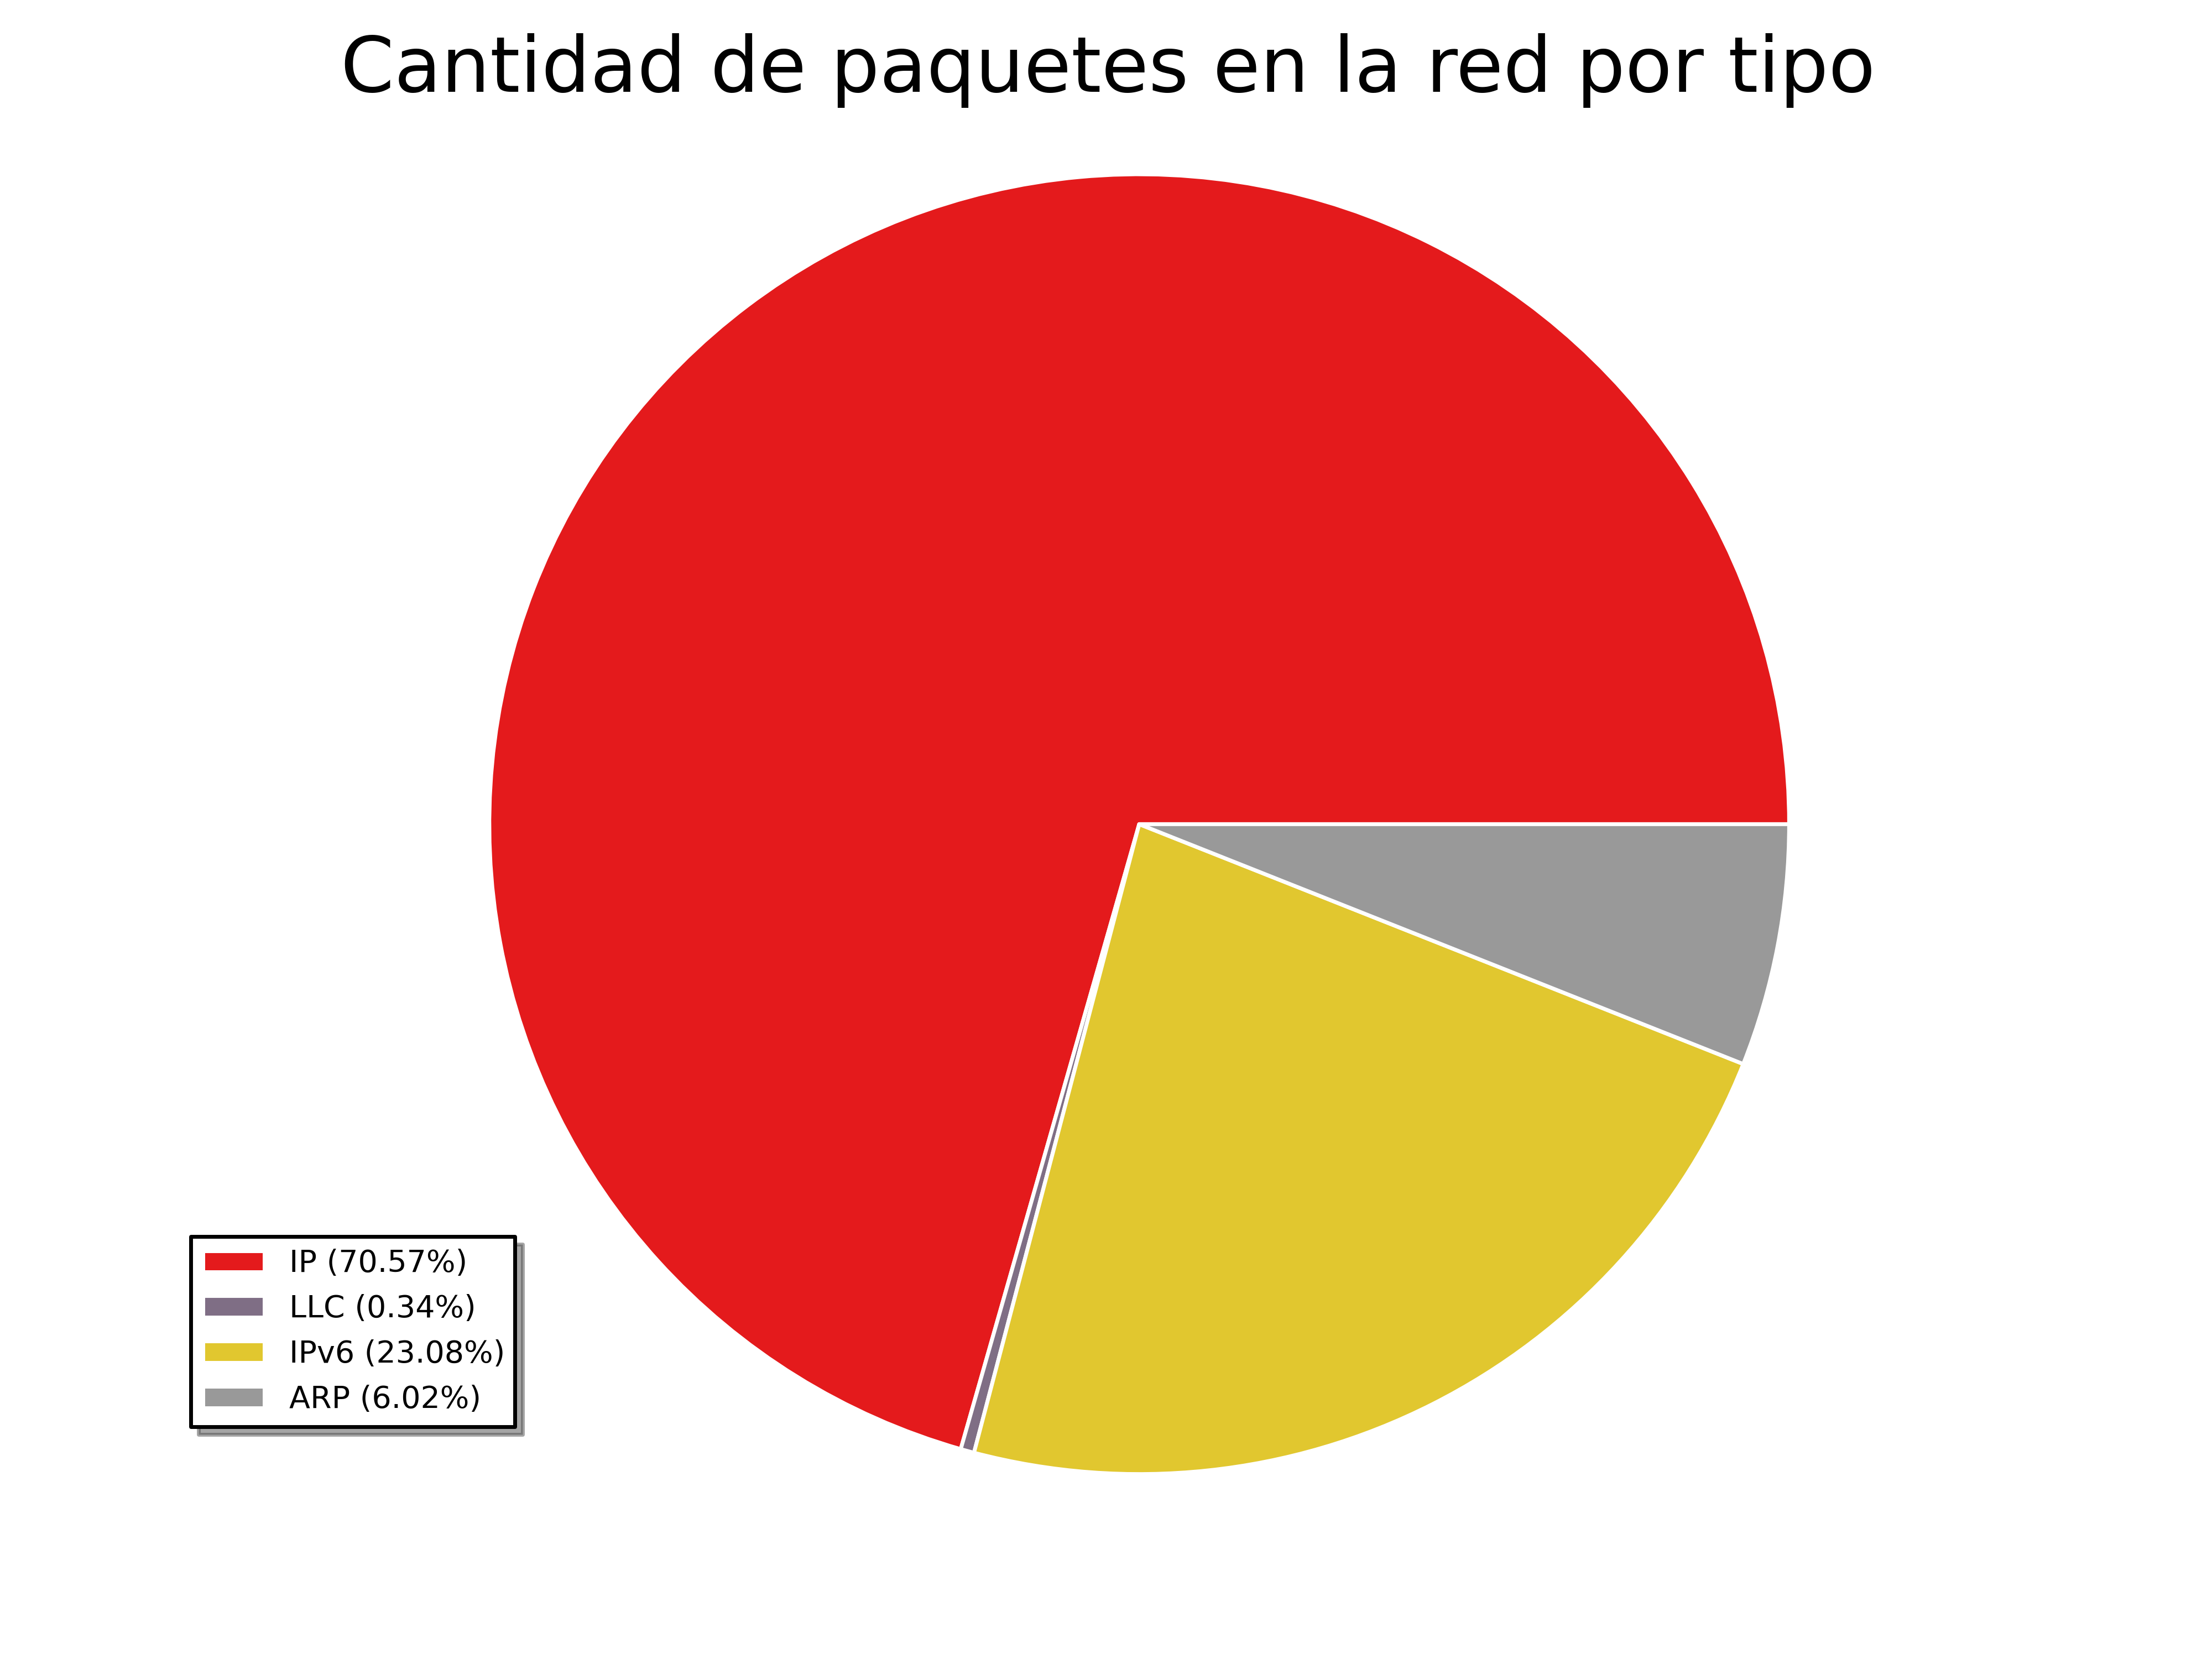
\includegraphics[width=\textwidth]{graficos/red_baufest_pie_type.png}
    \caption{Fuente $S$}
    \label{fig:red_baufest_pie_type}
  \end{minipage}
  \hfill
  \begin{minipage}[b]{0.48\textwidth}
    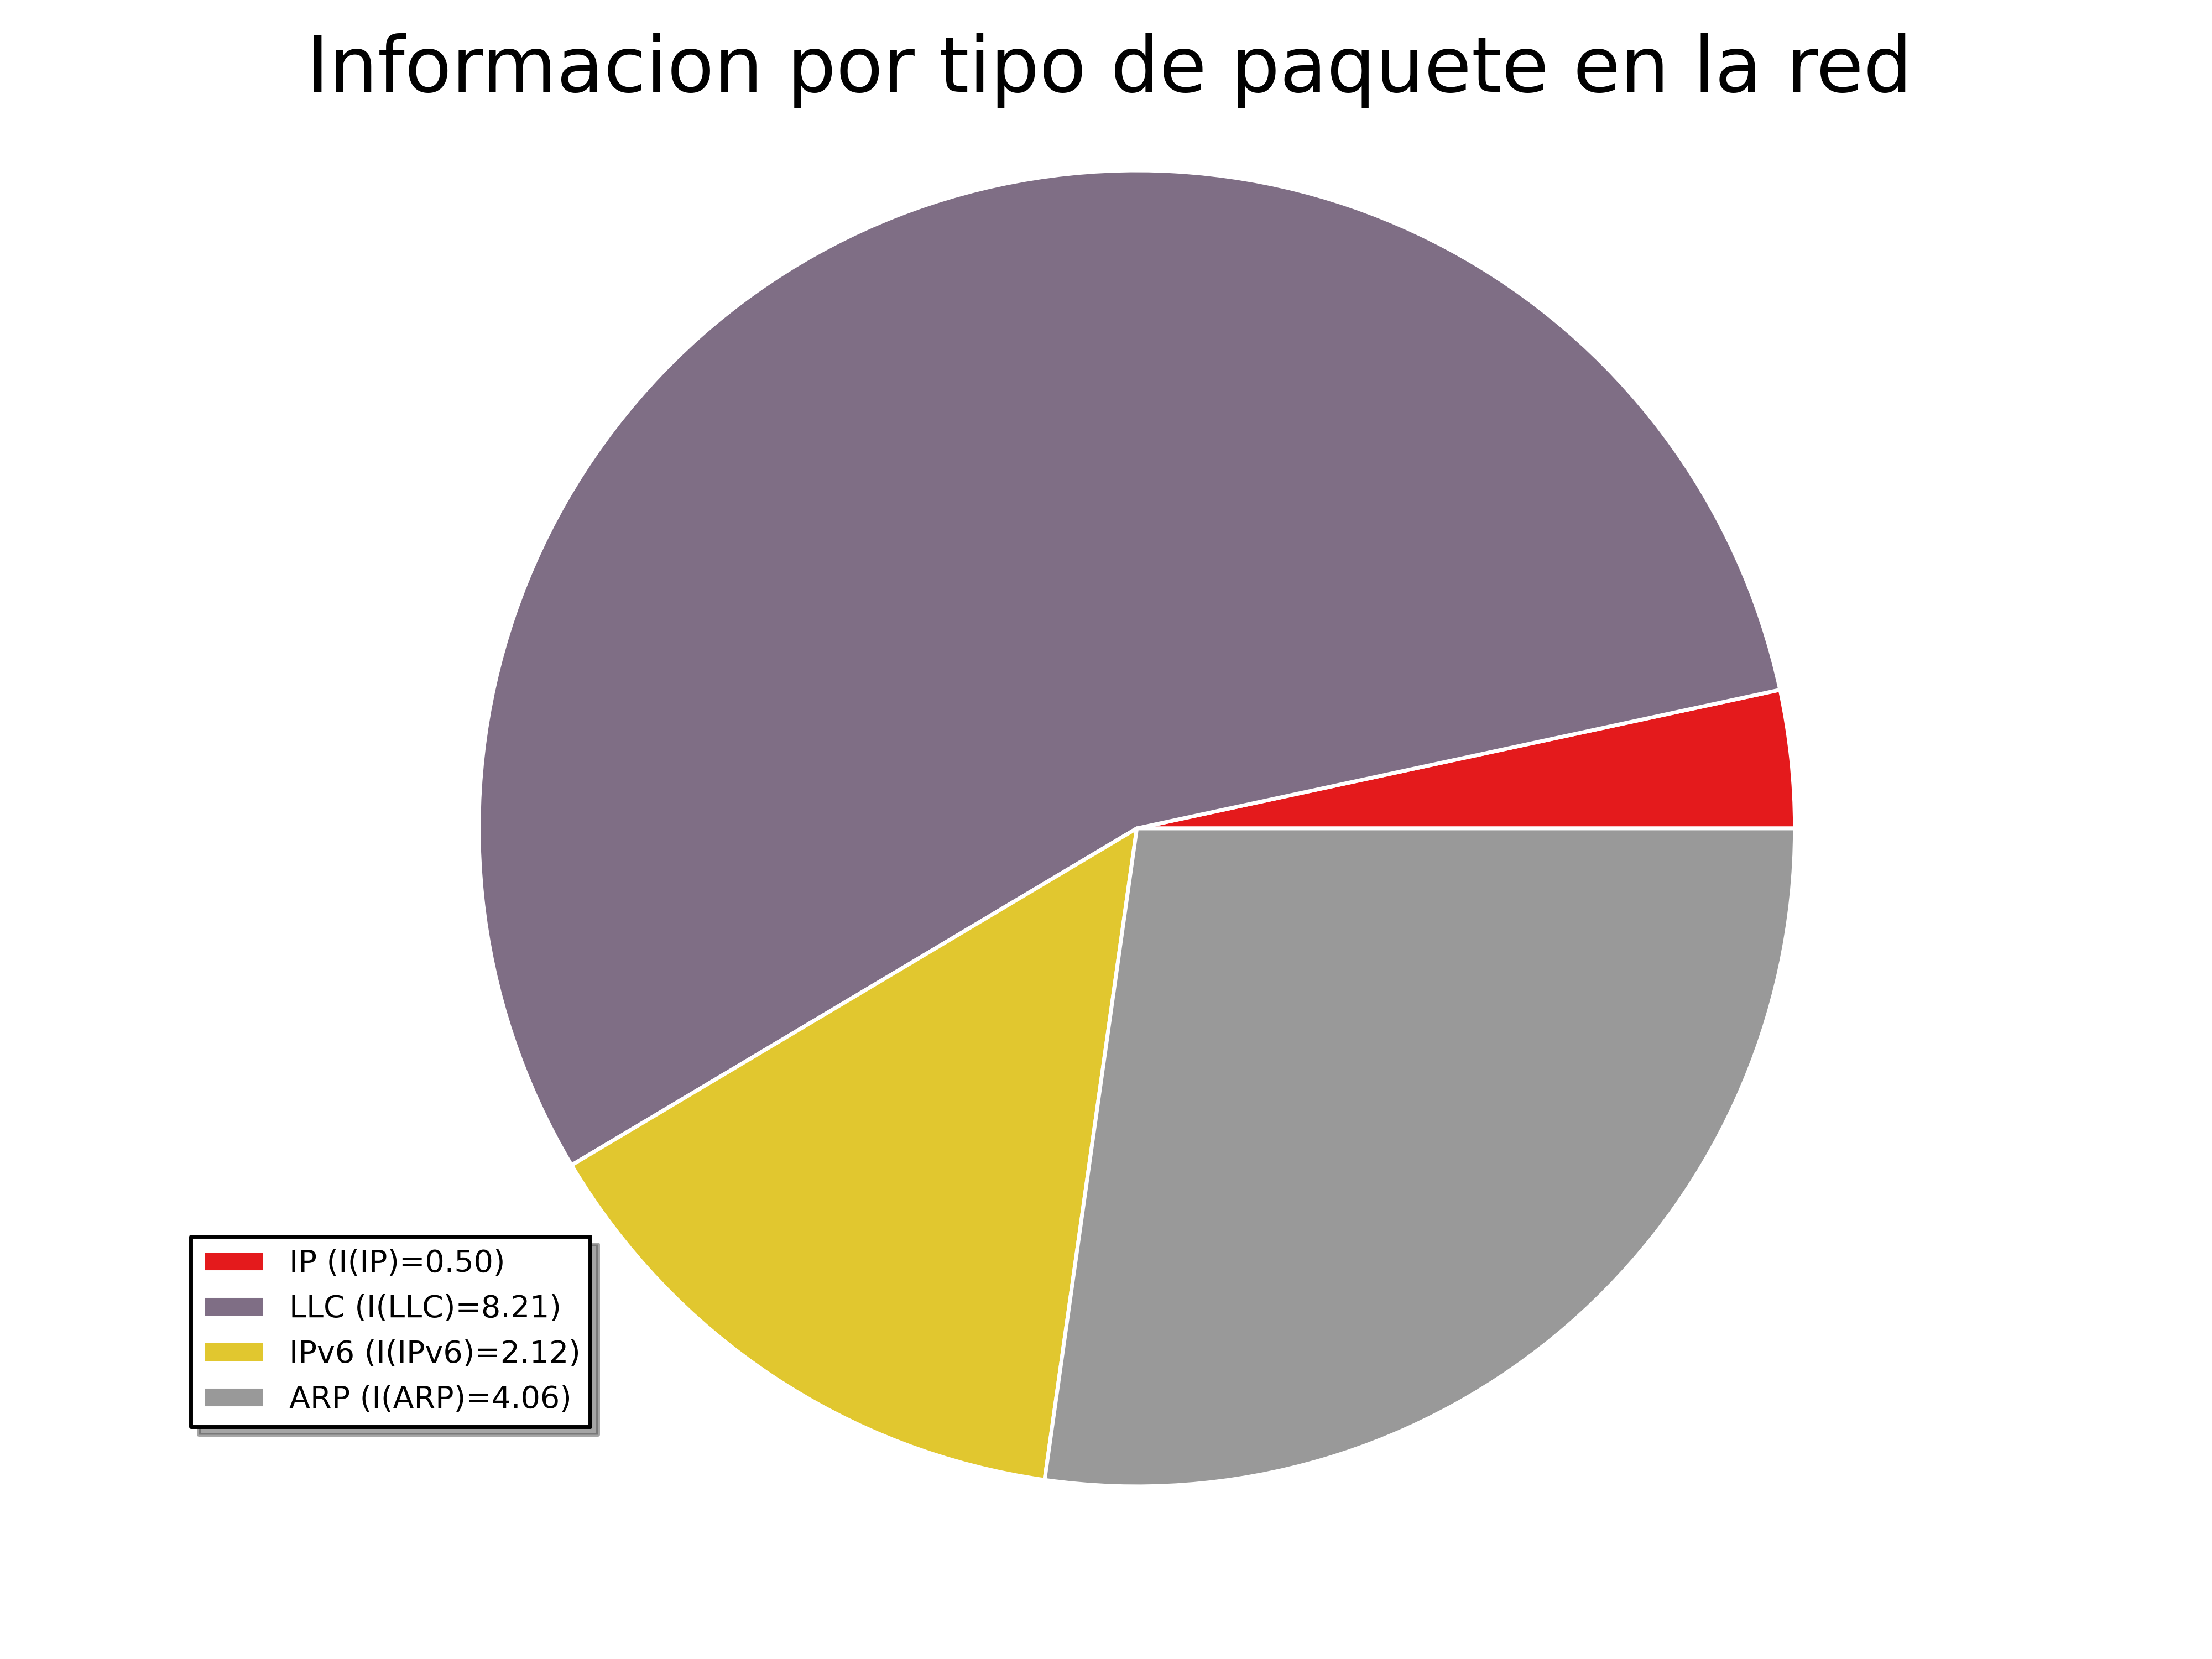
\includegraphics[width=\textwidth]{graficos/red_baufest_pie_type_information.png}
    \caption{Fuente $S$}
    \label{fig:red_baufest_pie_type_information}
  \end{minipage}
\end{figure}

En los gráficos Figura ~\ref{fig:red_baufest_pie_type}. y Figura ~\ref{fig:red_baufest_pie_type_information} se puede observar que el protocolo IPv4 es el mas frecuente. Pero también se observa gran cantidad de paquetes IPv6.
\\
Podemos ver que la cantidad de paquetes ARP, en comparación con IPv4 e IPv6, es baja. Sin embargo, en este caso, la proporción de paquetes ARP es mayor que en el caso de la red doméstica. 
\\
\\
\FloatBarrier

Veremos la relación entre la cantidad de paquetes y la información que proporciona cada nodo en la red para la fuente $S_1$. 

\begin{figure}[ht!]
  \centering
  \begin{minipage}[b]{0.48\textwidth}
    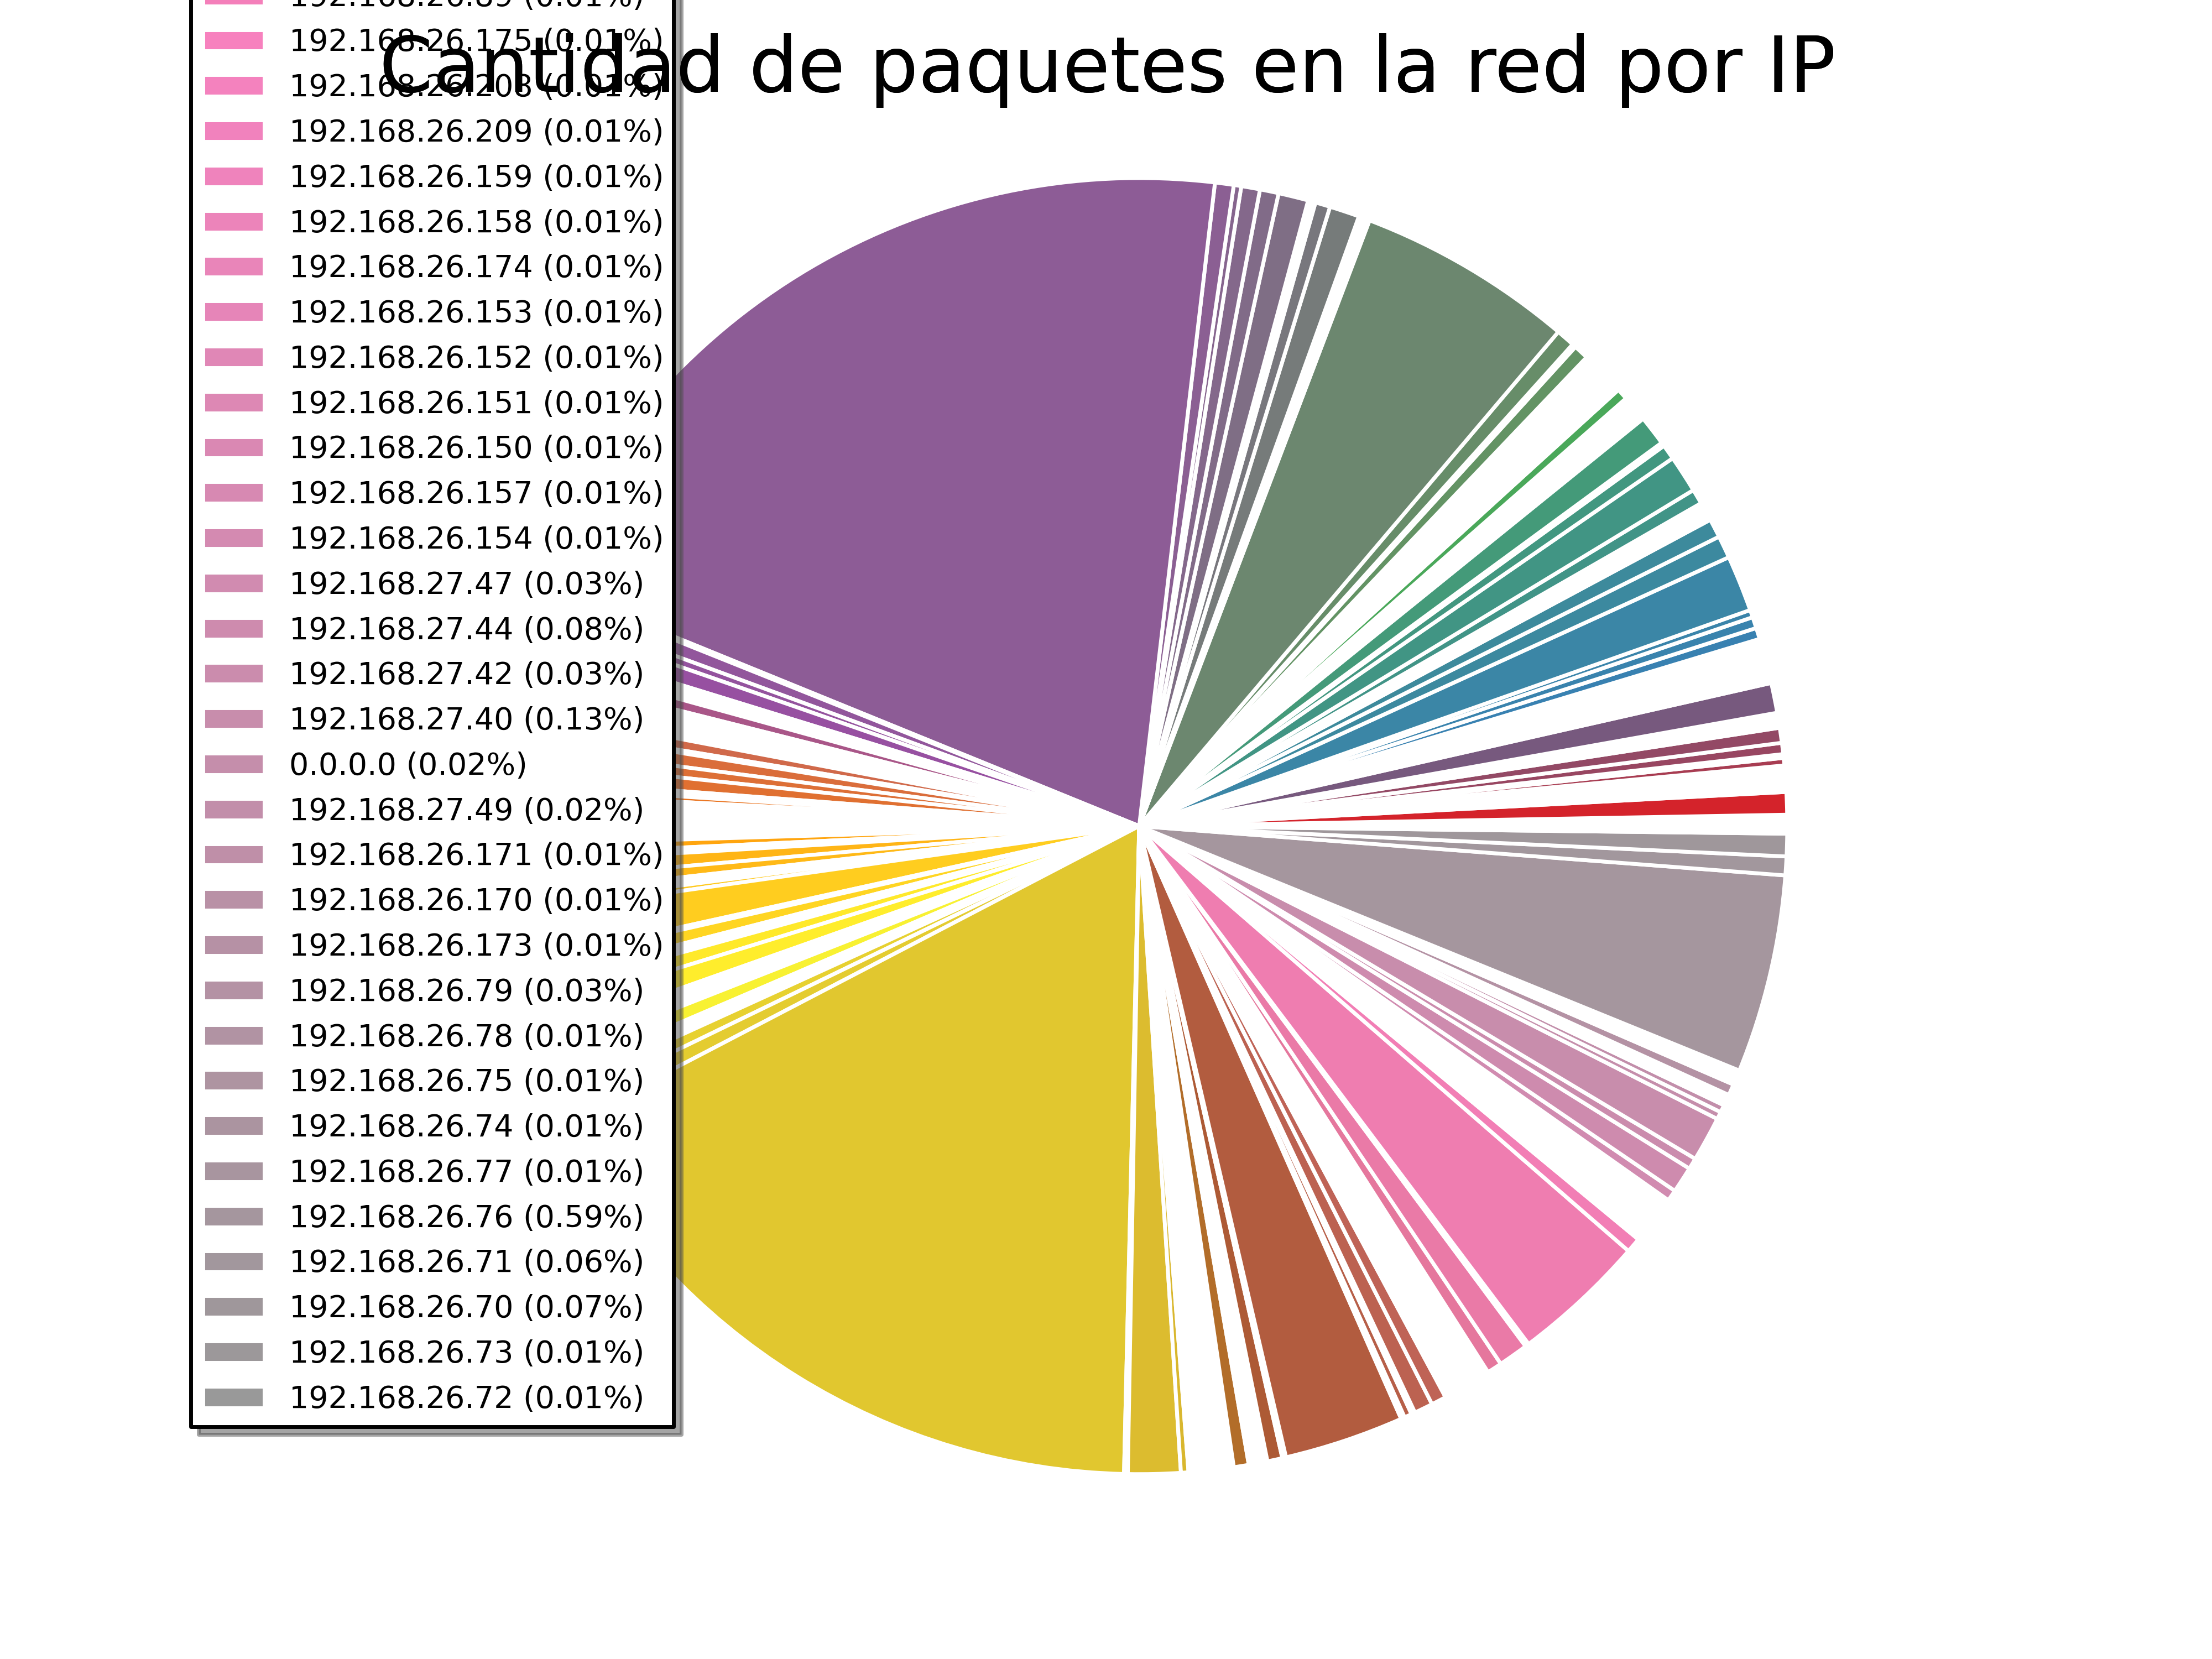
\includegraphics[width=\textwidth]{graficos/red_baufest_pie_arp.png}
    \caption{Fuente $S_1$}
    \label{fig:red_baufest_pie_arp}
  \end{minipage}
  \hfill
  \begin{minipage}[b]{0.48\textwidth}
    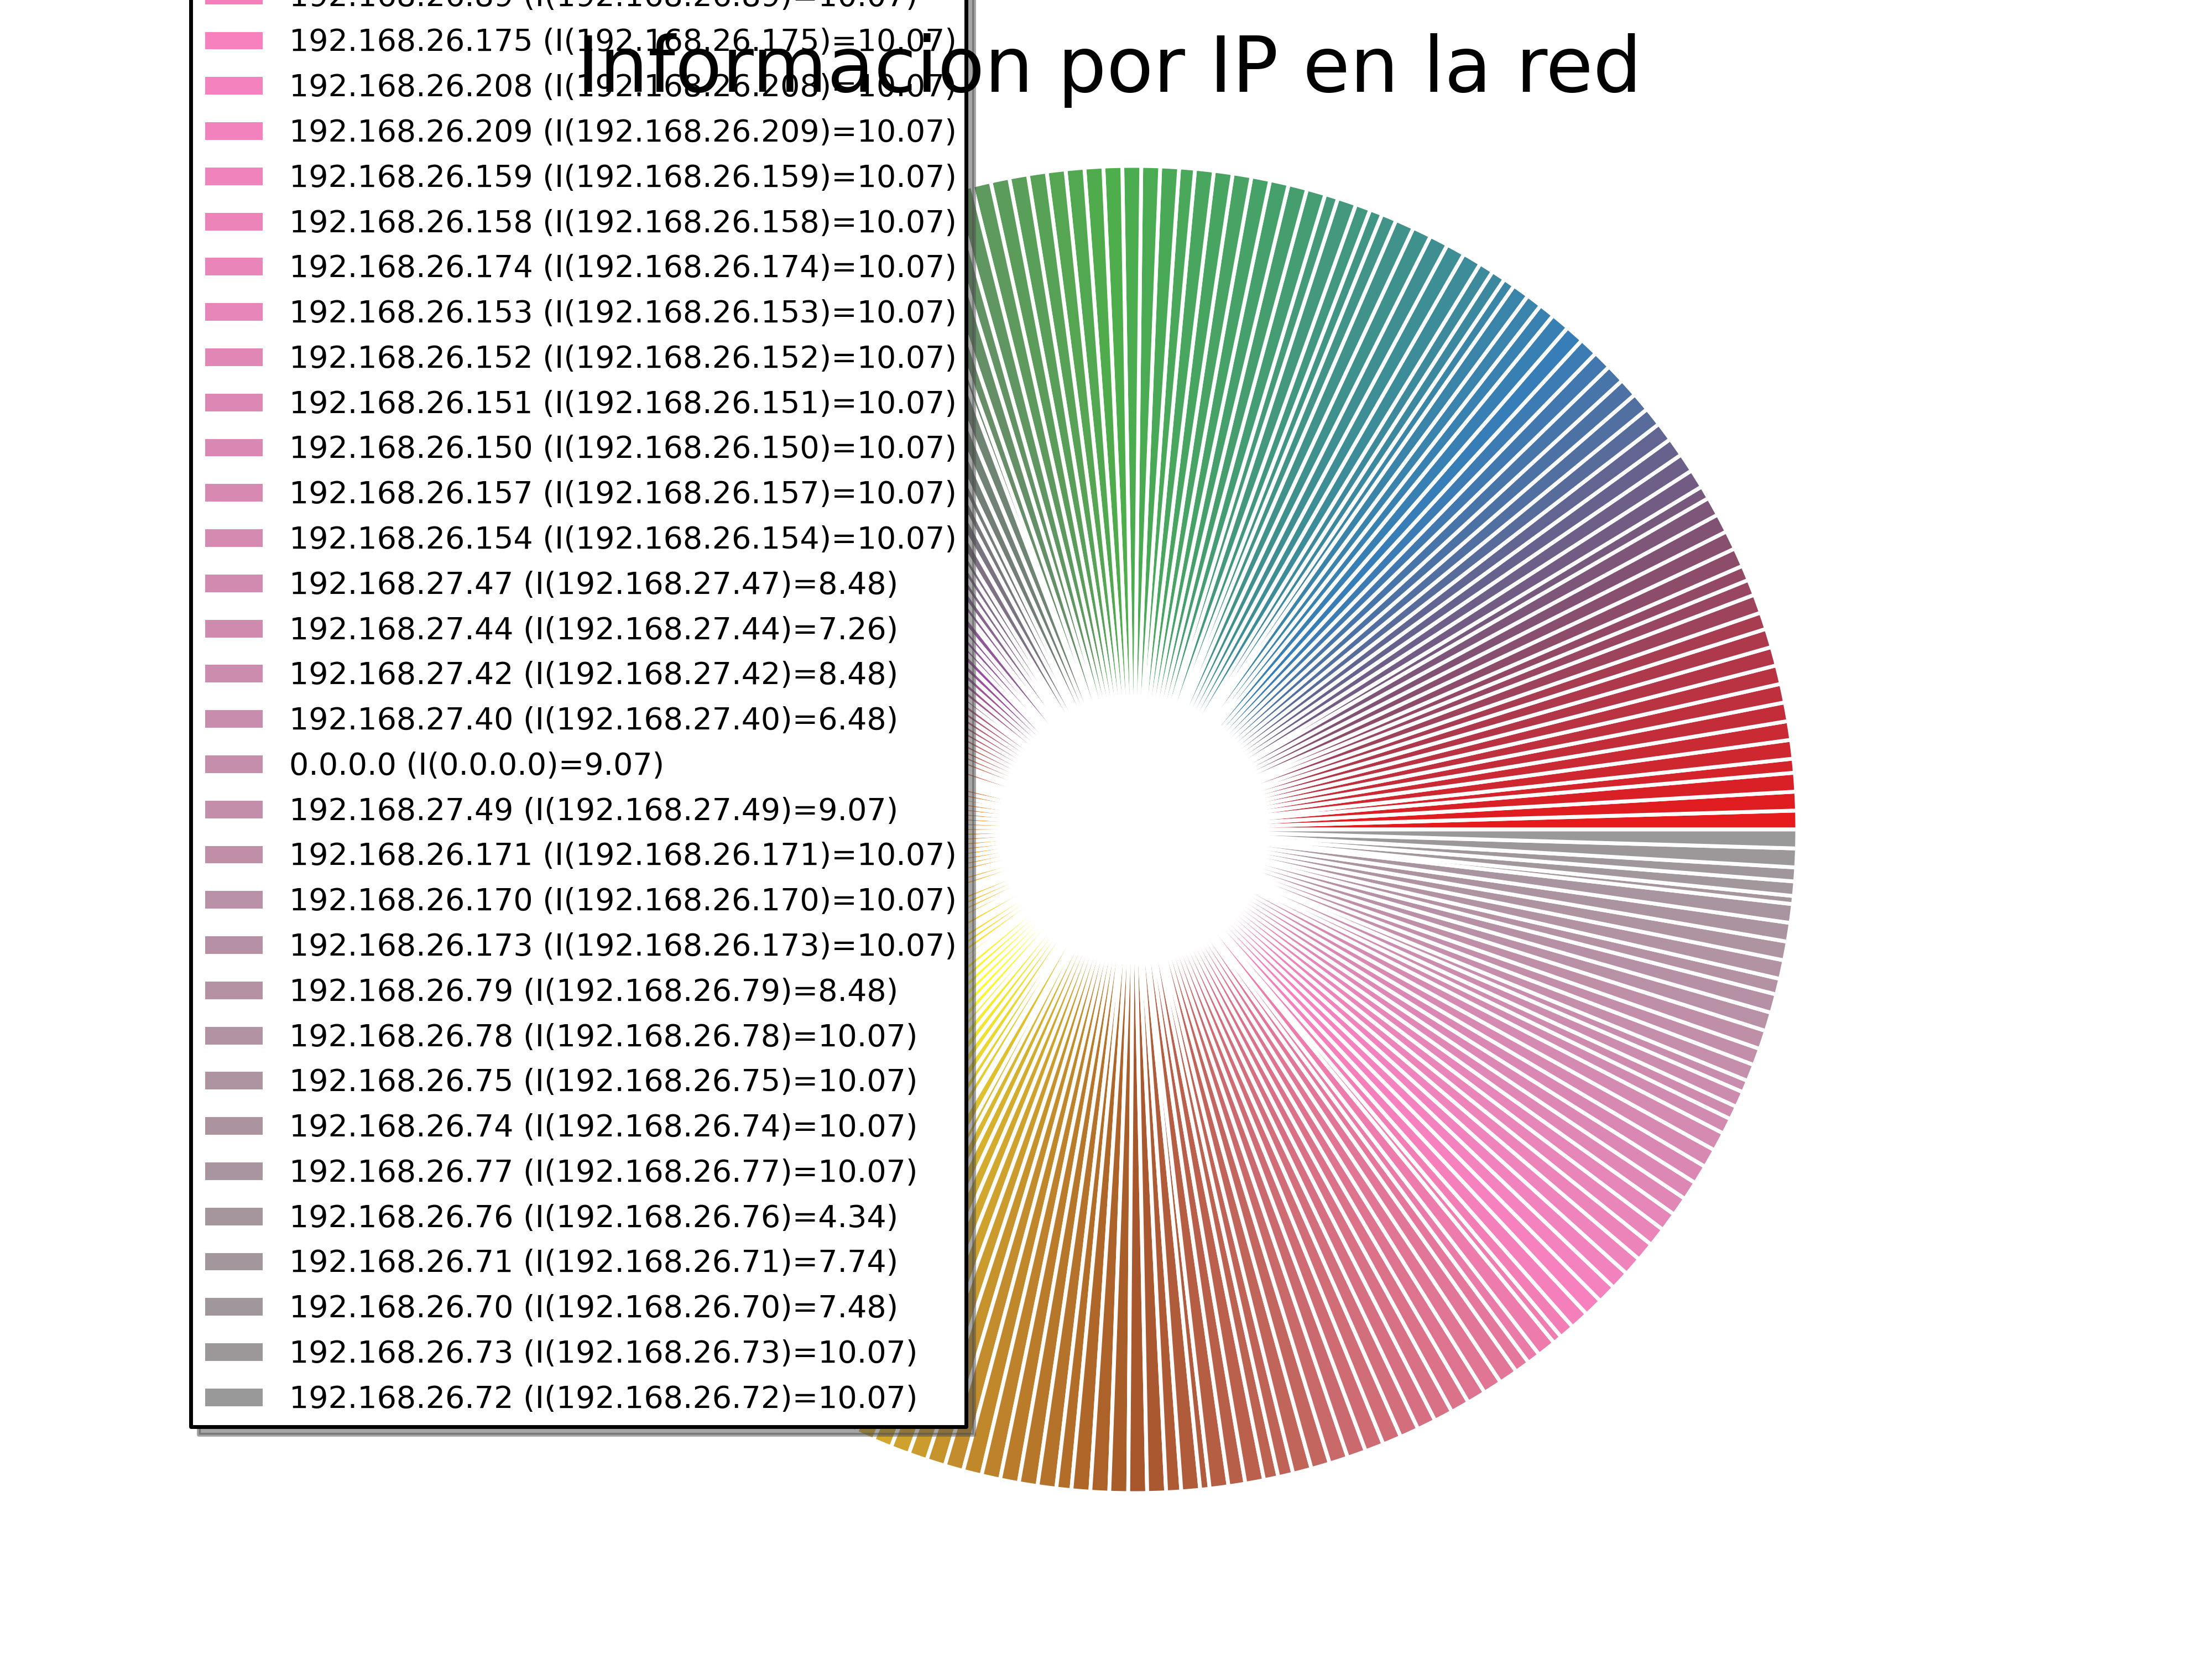
\includegraphics[width=\textwidth]{graficos/red_baufest_pie_arp_information.png}
    \caption{Fuente $S_1$}
    \label{fig:red_baufest_pie_arp_information}
  \end{minipage}
\end{figure}

Si bien se trata de una red grande, se puede ver en los gráficos Figura ~\ref{fig:red_baufest_pie_arp}. y Figura ~\ref{fig:red_baufest_pie_arp_information}. que hay dos nodos que distinguen del resto: El que tiene dirección IP 192.168.26.43 con el 0.2\% y el de IP 192.168.26.1 con el 0.17\%. Se presume que esos nodos deben ser routers. 

\FloatBarrier

\subsubsection{Análisis de la de entropía}

Vemos histogramas con cortes en los valores de entropía, tanto para las fuentes $S$ y $S_1$

\begin{figure}[ht!]
  \centering
  \begin{minipage}[b]{0.48\textwidth}
    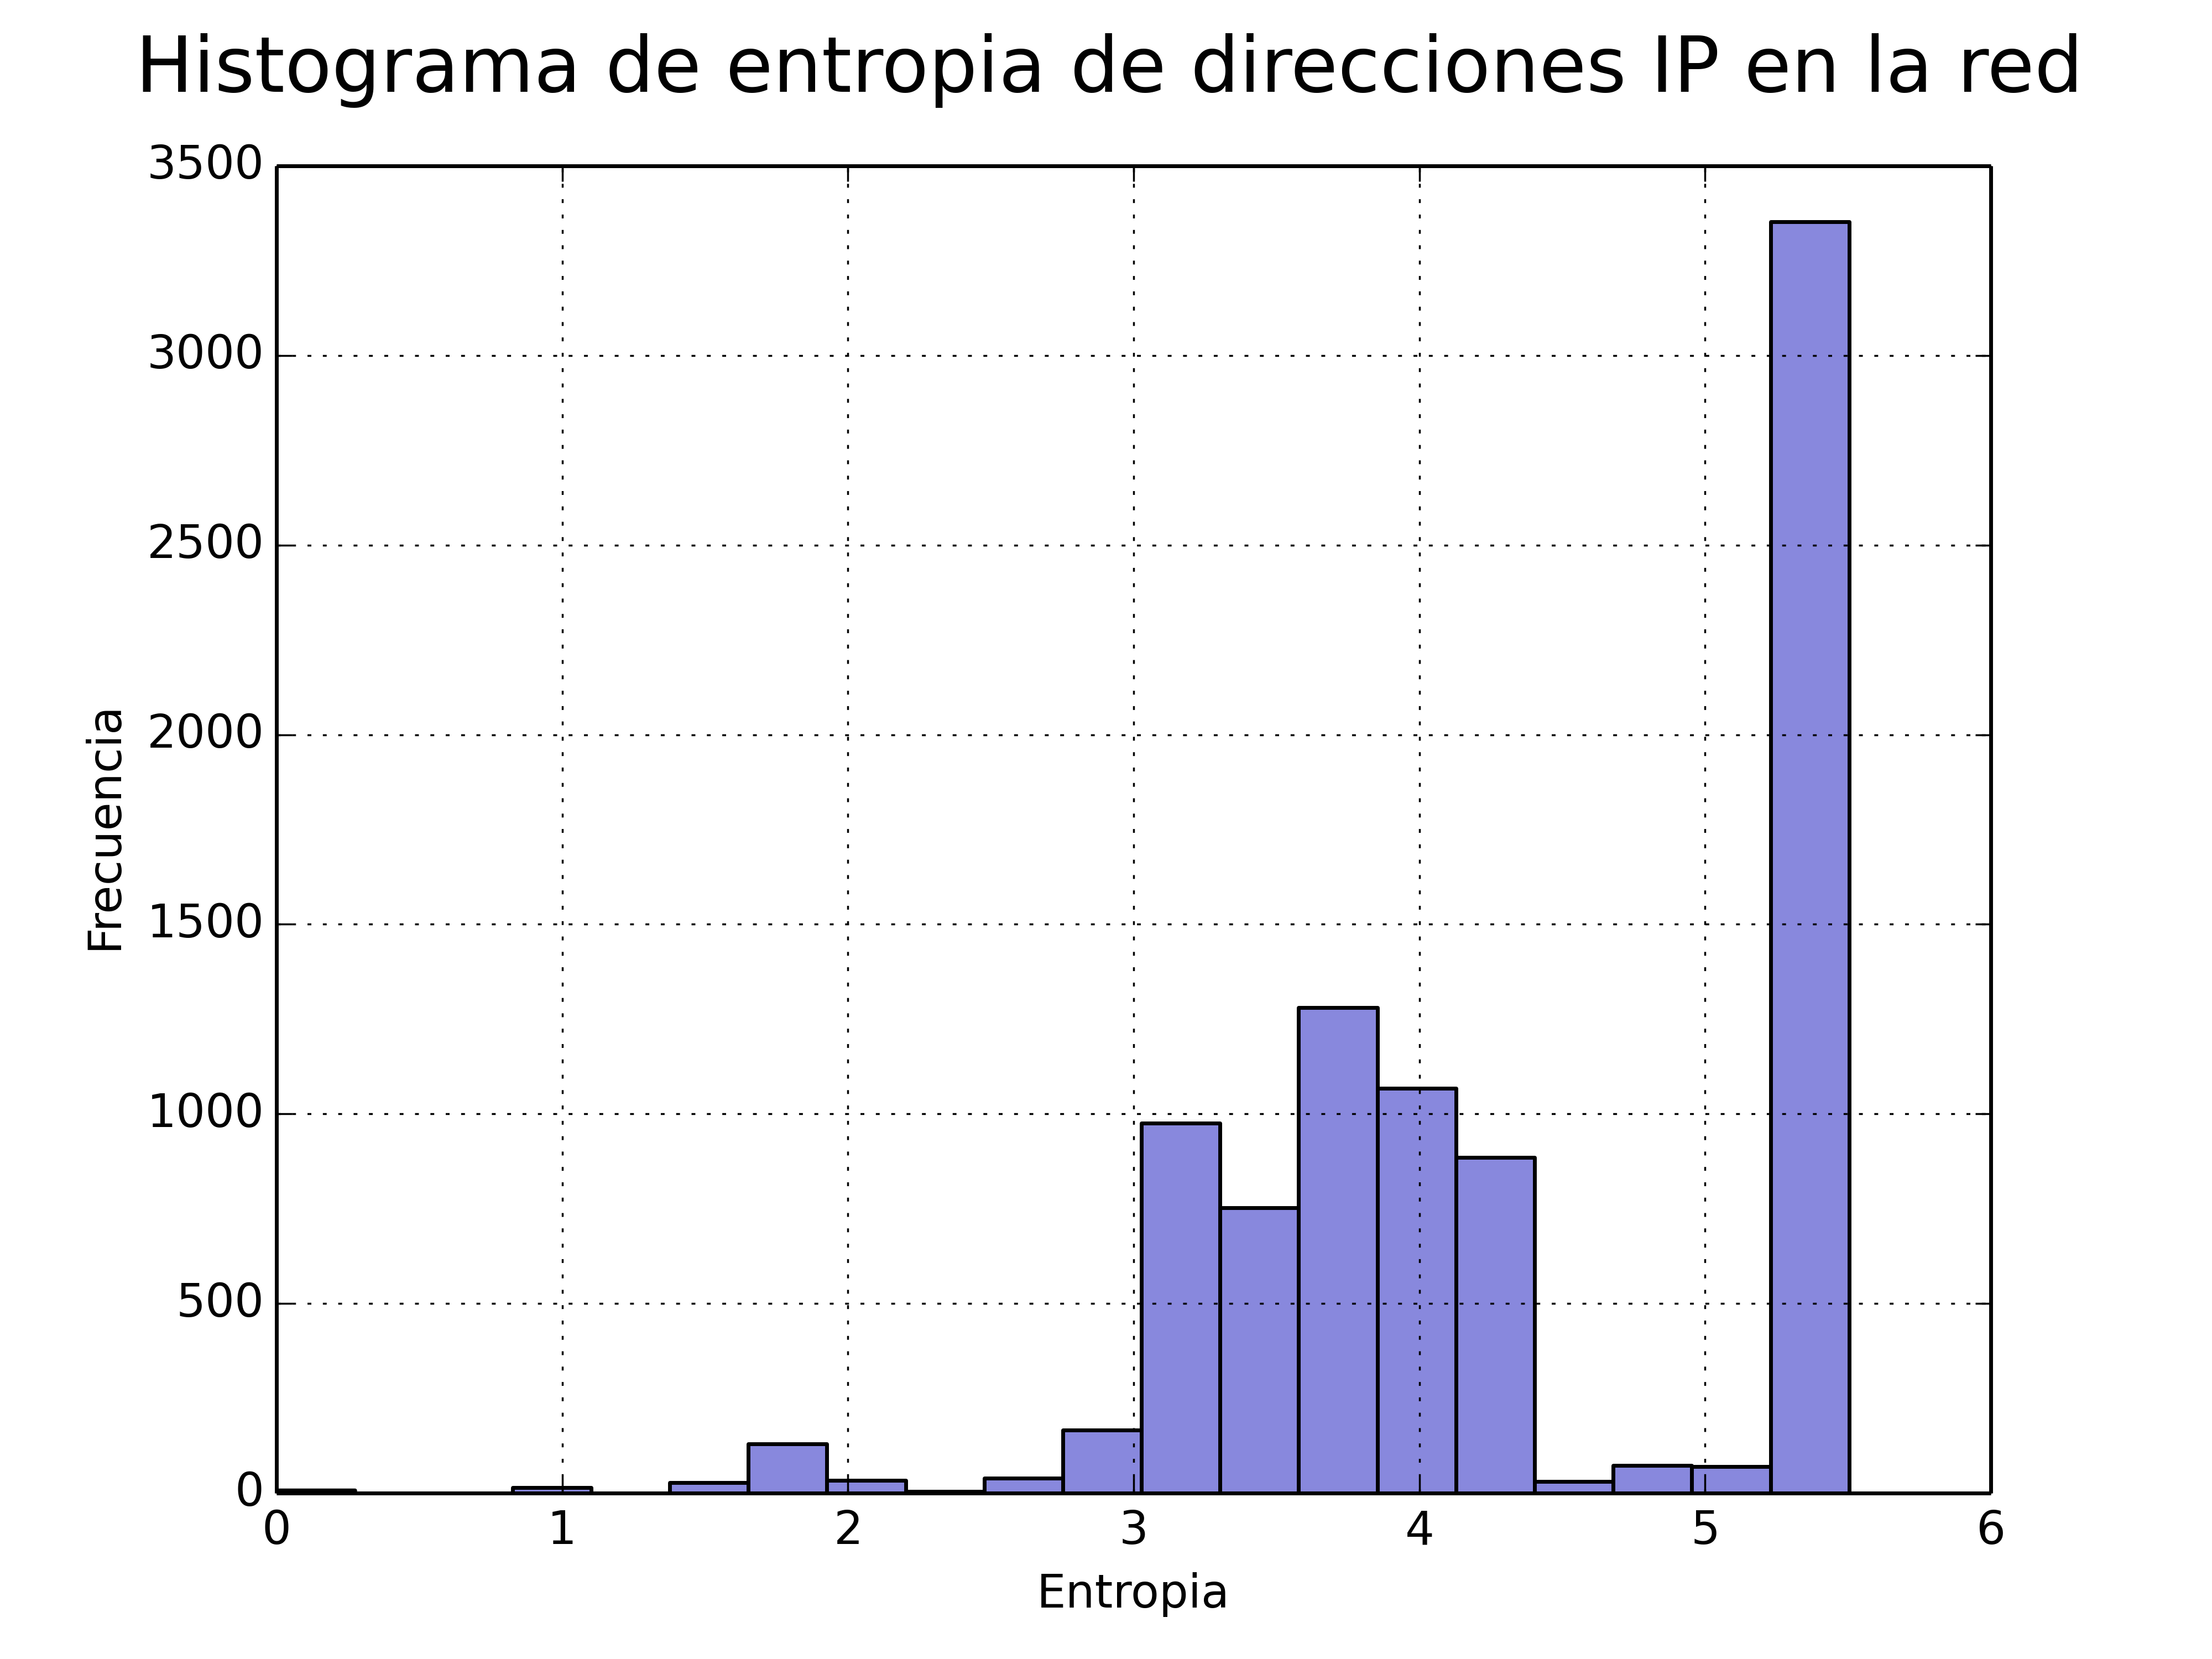
\includegraphics[width=\textwidth]{graficos/red_baufest_hist_arp.png}
    \caption{Fuente $S$}
    \label{fig:red_baufest_hist_arp}
  \end{minipage}
  \hfill
  \begin{minipage}[b]{0.48\textwidth}
    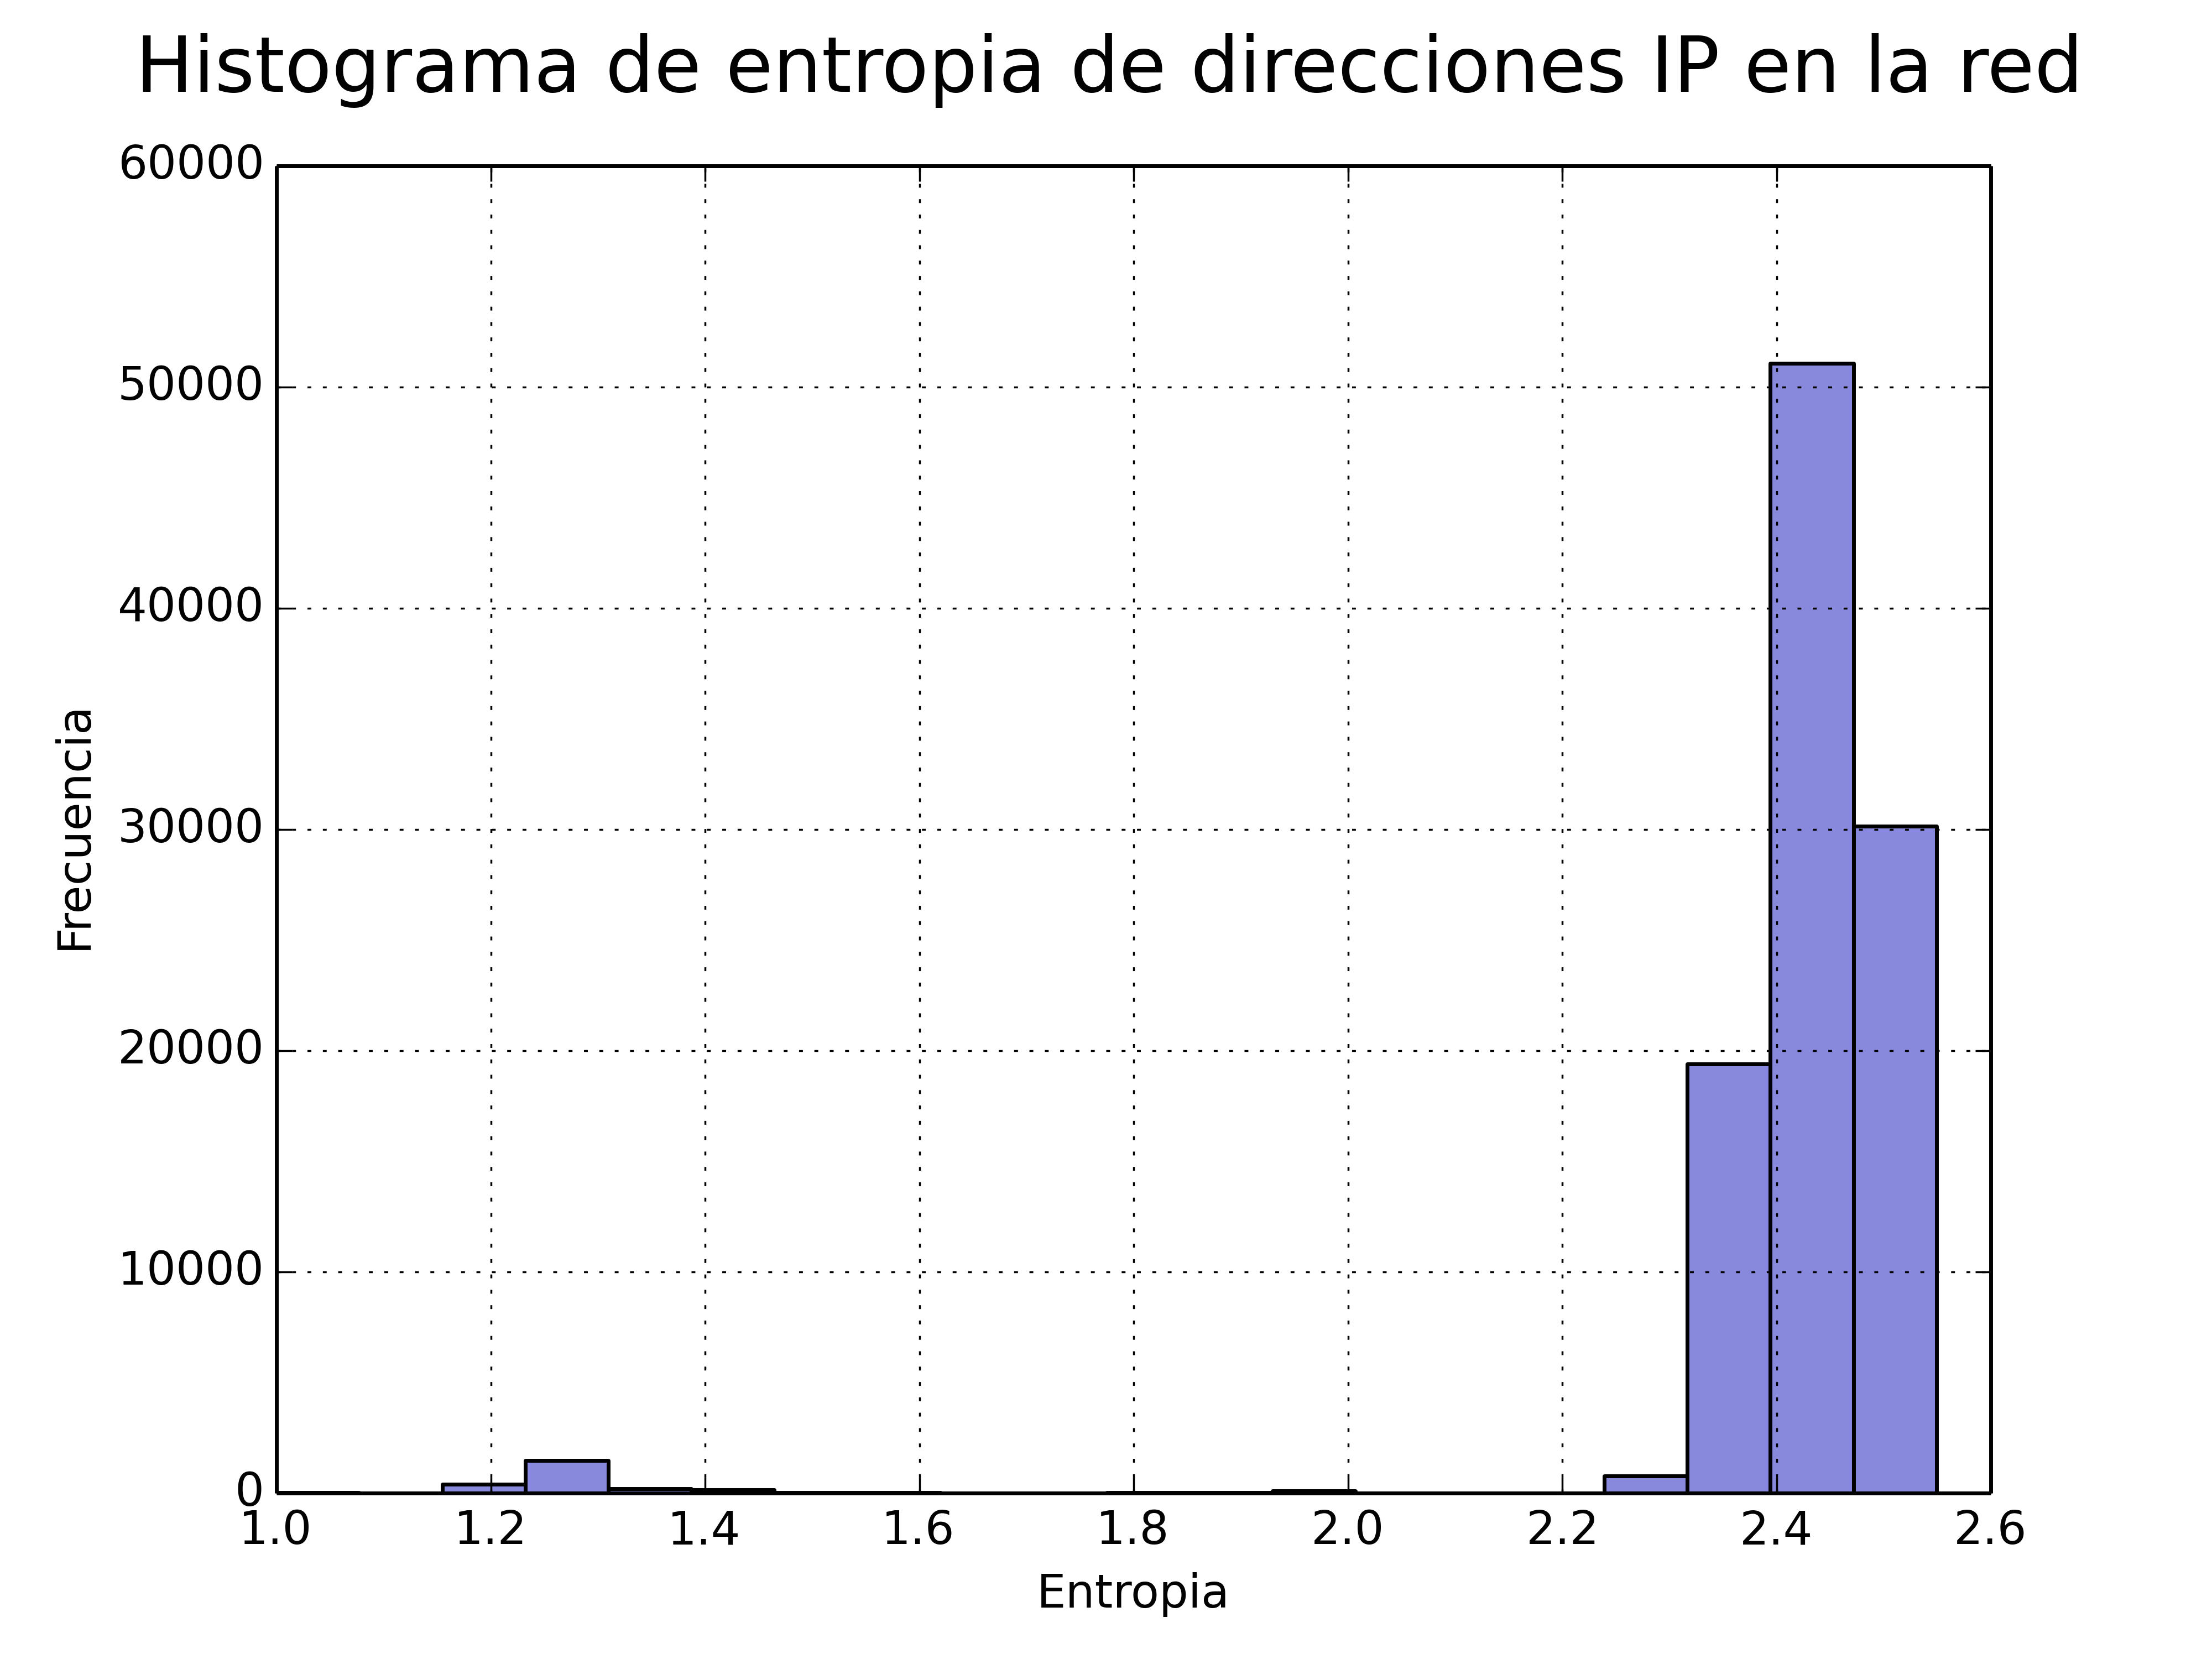
\includegraphics[width=\textwidth]{graficos/red_domestica_hist_arp.png}
    \caption{Fuente $S_1$}
    \label{fig:red_domestica_hist_arp}
  \end{minipage}
\end{figure}